\textbf{Цель работы:} изучение петель гистерезиса различных ферромагнитных
материалов в переменных полях.\\\indent
\textbf{Оборудование:} автотрансформатор, понижающий трансформатор, интегрирующая цепочка, амперметр, вольтметр, электронный
осциллограф, делитель напряжения, тороидальные образцы с двумя обмотками.

\section*{Теоретические сведения}

\begin{wrapfigure}{l}{0.5\linewidth}
    \centering
    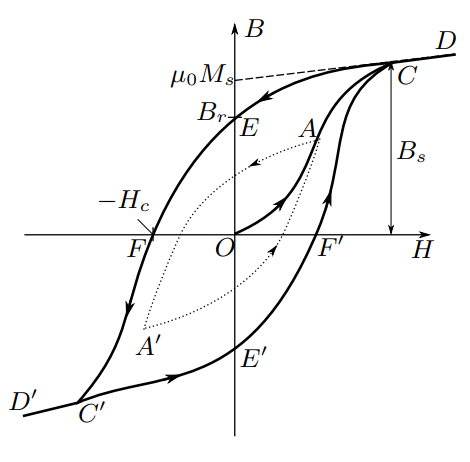
\includegraphics[width=6cm]{images/gisterezis.png}
    \caption{Петля гистерезиса ферромагнетика}
\end{wrapfigure}

\indent Магнитная индукция $B$ и напряжённость поля $H$ в ферромагнитном материале неоднозначно связаны между собой: индукция зависит
не только от напряжённости, но и от предыстории образца.\\
\indent Если к ферромагнитному образцу прикладывать переменное внешнее
магнитное поле, то его состояние на плоскости $HB$ будет изменяться
по замкнутой кривой — петле гистерезиса. Пересечение предельной петли с вертикальной осью соответствует остаточной индукции $B_r$, пересечение с горизонтальной осью - коэрцитивному полю $H_c$.
\\
\section*{Экспериментальная установка}
\indent Напряжение от сети (220 В, 50Гц) с помощью трансформаторного блока Т, состоящего из автотрансформатора и реостата $R_1$, включенного как потенциометр, подается на намагничивающую обмотку $N_0$ исследуемго образца.

\begin{figure}[h!]
    \centering 
    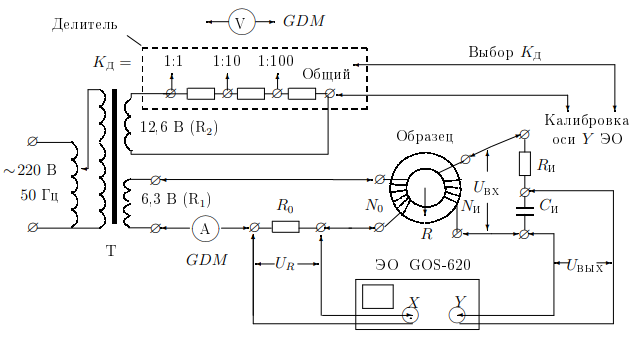
\includegraphics[width=15cm]{images/setup.png}
    \caption{Схема установки для намагничивания образцов}
\end{figure}

\indent В цепь катушки, на которую подается напряжение $U_0 = 6.3$ В, последовательно включены амперметр А и резистор $R_0$. Напряжение на $R_0$ подается на канал $X$ осциллографа. Напряженность $H$ в образце прямо пропорциональна току $I_0$ по теореме о циркуляции: 
\begin{equation}
    H = \frac{IN_0}{2\pi R} \label{eq:H}
\end{equation}

\indent Чтобы измерить магнитную индукцию $B$, с измерительной обмотки $N_и$ на вход интегрирующей $RC$-цепочки подается напряжение $U_и = U_{\text{вх}}$, пропорциональное $dB/dt$, а с выхода снимается напряжение $U_C = U_{\text{вых}}$, пропорциональное $B$. Оно же и подается на канал $Y$ осциллографа.
\begin{equation}
    B = \frac{R_{\text{и}}C_{\text{и}}}{S N_{\text{и}}}U_{\text{вых}} \label{eq:B}
\end{equation}
\indent На экране появляется замкнутая кривая в некотором масштабе. Чтобы получить численные данные, необходимо откалибровать каналы $X$ и $Y$ осциллографа.\\
\indent \textbf{Калибровка канала $X$ ЭО} проводится с помощью амперметра при закороченной обмотке $N_0$. Тогда амперметр измеряет эффективное значение силы тока $I_{\text{эф}}$. Ширина горизонтальной развертки на экране  ЭО ($2x$) соответствует удвоенной амплитуде напряжения на $R_0$. Тогда чувствиетельность кнала $X$ $K_X$:
\begin{equation}
    K_X = 2\sqrt{2}R_0 I_{\text{эф}}/(2x) \label{eq:Kx}
\end{equation}

\indent \textbf{Калибровка канала $Y$ ЭО} проводится с помощью вольтметра. Сигнал с обмотки понижающего трансформатора подаетя на делитель напряжения. Часть этого напряжения снимается с делителя с коэффициентом деления $K_{Д}$ (1:100) и подается на вход $Y$ ЭО. Вольтметр измеряет напряжение $U_{\text{эф}}$ на этих же клеммах делителя. Если $2y$ - длина вертикальной прямой на ЭО, то тогда чувствиетельность кнала $Y$ $K_Y$:
\begin{equation}
    K_Y = 2\sqrt{2}U_{\text{эф}}/(2y) \label{eq:Ky}
\end{equation}
\indent \textbf{Измерение параметров интегрирующей ячейки.} C обмотки на вход $RC$-цепочки подается синусоидальное напряжение $U_{\text{вх}}$ c частотой $\nu = \omega / 2\pi = 50$ Гц. На канал $Y$ ЭО поочередно подаются сигналы со входа и выхода $RC$-цепочки. Тогда измерив амплитуды этих сигналов можно рассчитать постоянную времени $\tau = RC$ как:
\begin{equation}
    \tau = RC = \frac{U_{\text{вх}}}{\omega U_{\text{вых}}} \label{eq:tau}
\end{equation}
\section*{Экспериментальные данные и вычисления}

\begin{wraptable}{l}{0.4\linewidth}
    \centering 
    \begin{tabular}{|c|c|c|}
        \hline
        $R_{\text{и}}$, кОм & $C_{\text{и}}$, мкФ & $R_0$, Ом \\\hline 
        20 & 20 & 0.22\\\hline
    \end{tabular}
    \caption{Параметры установки}
\end{wraptable}

\indent Для изучения гистерезиса в работе использовались тороиды из кремнистого железа, пермаллоя и феррита. Для них были получены петли гистерезиса и вычислены некоторые параметры. 
\\
\begin{table}[h!]
    \centering
    \begin{tabular}{|c|c|c|c|c|}
        \hline
        Материал            & $N_0$ & $N_{\text{и}}$& $S$, cм$^2$& $2\pi R$, cм  \\\hline 
        Кремнистое железо   & 20    & 200           & 2          & 11            \\\hline
        Пермаллой           & 15    & 300           & 0.66       & 14.1          \\\hline
        Феррит              & 45    & 400           & 3          & 25            \\\hline
    \end{tabular}
    \caption{Параметры установки для различных материалов}
\end{table}

\begin{figure}[h!]
    \begin{subfigure}[b]{0.55\linewidth}
        \centering
        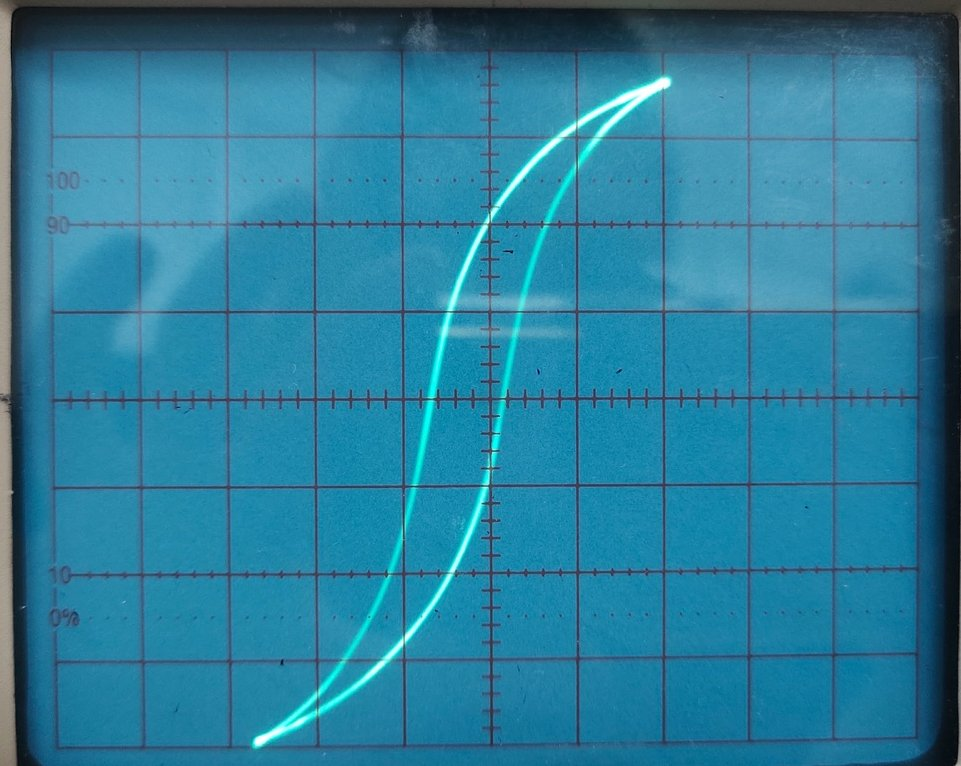
\includegraphics[width=9cm]{images/kremni.jpg}
        \caption{Предельная петля гистерезиса кремнистого железа}
    \end{subfigure}
    \begin{subfigure}[b]{0.5\linewidth}
        \centering
        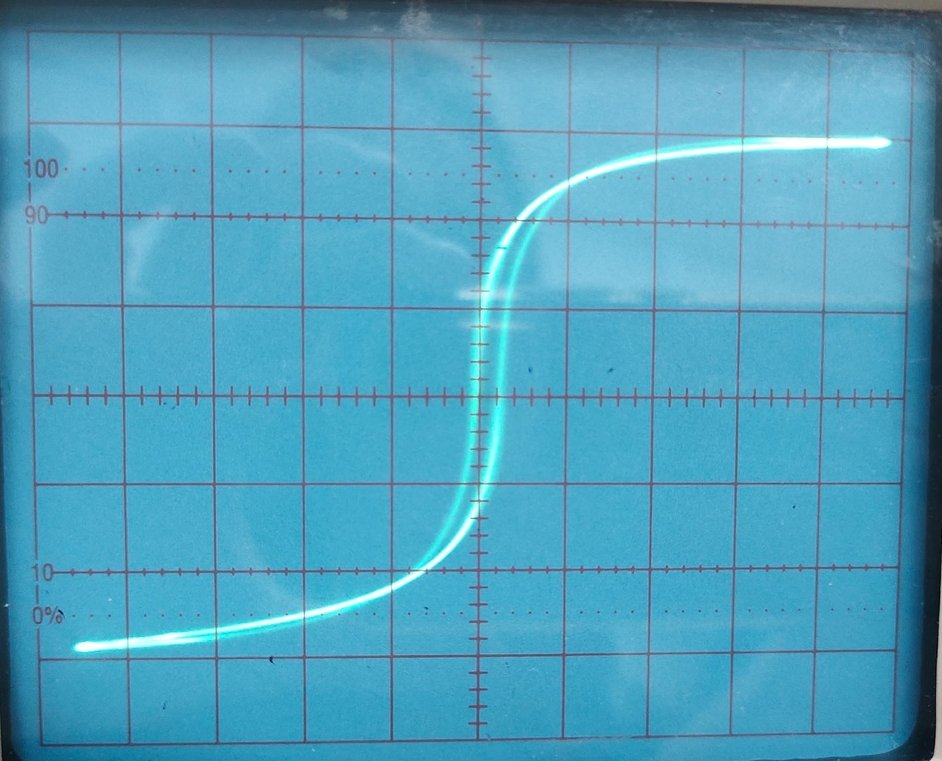
\includegraphics[width=9cm]{images/ferrit.jpg}
        \caption{Предельная петля гистерезиса феррита}
    \end{subfigure}
\end{figure}

\begin{table}[h!]
    \centering
    \begin{tabular}{|c|c|c|c|c|}
        \hline
        Материал & $2X_s$ дел & $2Y_s$, дел & $2X_c$, дел & $2Y_r$, дел \\\hline 
        Кремнистое железо    & 24 $\pm 0.5$ & 38.5 $\pm 0.5$ & 4.5 $\pm 0.5$ & 14 $\pm 0.5$ \\\hline
        Пермаллой            & 20 $\pm 0.5$ & 18   $\pm 0.5$ & 10  $\pm 0.5$ & 18 $\pm 0.5$ \\\hline
        Феррит               & 46 $\pm 0.5$ & 29   $\pm 0.5$ & 1.5 $\pm 0.5$ & 11 $\pm 0.5$ \\\hline
    \end{tabular}
    \caption{Индукция и напряженность магнитного поля в разных ферромагнетиках}
\end{table}
\newpage

\begin{figure}[h!]
    \begin{subfigure}[b]{0.5\linewidth}
        \centering
        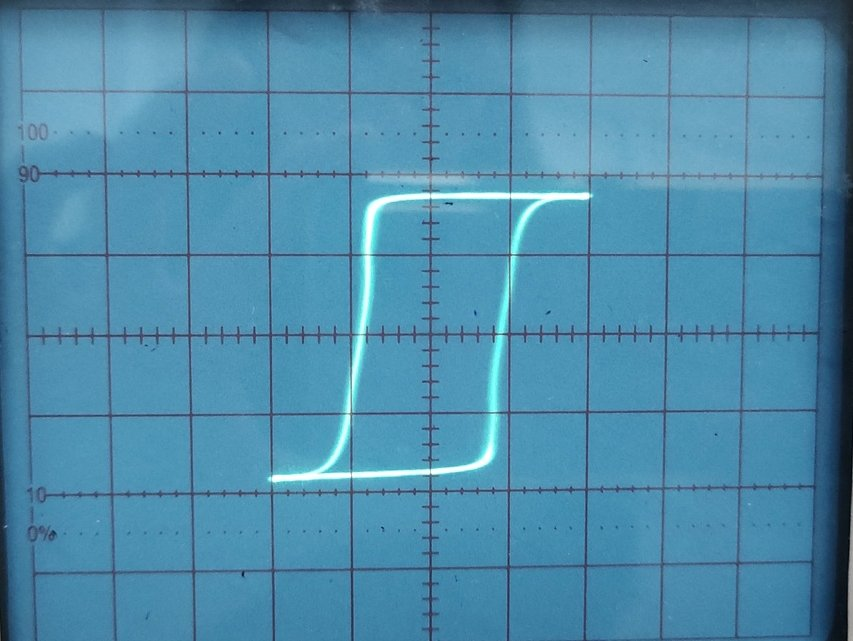
\includegraphics[width=9cm]{images/permalloy.jpg}
        \caption{Предельная петля гистерезиса пермаллоя}
    \end{subfigure}
    \hfill
    \begin{subfigure}[b]{0.45\linewidth}
        \centering
        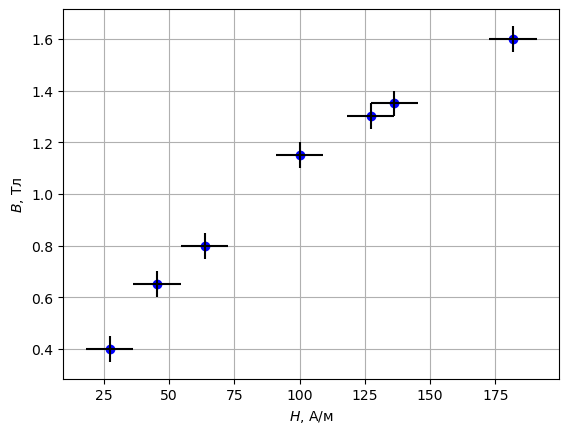
\includegraphics[width=9cm]{images/plot1.png}
        \caption{Начальная кривая намагничивания для крем. железа}
    \end{subfigure}
    \vfill
    \begin{subfigure}[b]{0.5\linewidth}
        \centering
        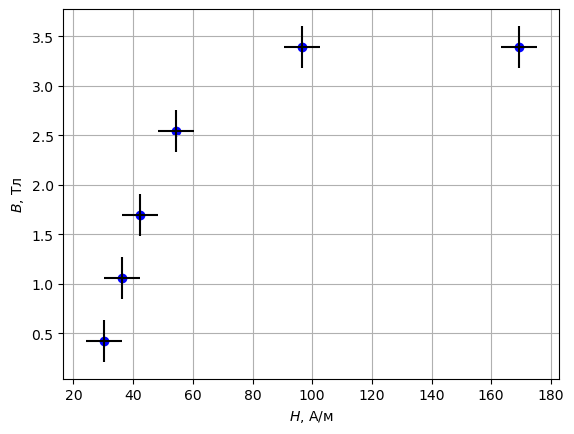
\includegraphics[width=9cm]{images/plot2}
        \caption{Начальная кривая намагничивания для пермаллоя}
    \end{subfigure}
    \hfill
    \begin{subfigure}[b]{0.45\linewidth}
        \centering
        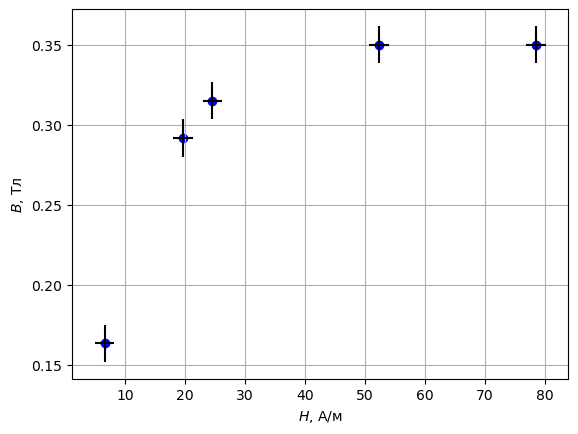
\includegraphics[width=9cm]{images/plot3.png}
        \caption{Начальная кривая намагничивания для феррита}
    \end{subfigure}
\end{figure}
\\
По начальным кривым намагничиваня оценим максимальные значения дифференциальной магнитной проницаемости $\mu_{\text{диф}} = \frac{1}{\mu_0}\frac{dB}{dH}\vert_{H = 0}$.

\begin{table}[h!]
    \centering
    \begin{tabular}{|c|c|c|c|c|}
        \hline
        Материал             & $B_s$, Тл & $H_c$, А/м & $\mu_{\text{нач}} \cdot 10^{3}$ & $B_r$, Тл   \\\hline 
        Кремнистое железо    & 1.9 $\pm$ 0.5  & 63\pm9    & 11 \pm 3 & 0.7\pm0.05  \\\hline
        Пермаллой            & 3.8 $\pm$ 0.2  & 48\pm6    & 11 \pm 4 & 3.8\pm0.2\\\hline
        Феррит               & 0.34 $\pm$ 0.05 & 1.6\pm0.7 & 20\pm2 & 0.12\pm 0.01\\\hline
    \end{tabular}
    \caption{Результаты вычислений\label{Tab:results}}
\end{table}
\newpage

\indent Теперь по формуле \ref{eq:tau} посчитаем постоянную времени интегрирующей цепочки и сравним результаты с значением $\tau_0 = C_{\text{и}}R_{\text{и}} = 0.4$ с. 
\\ $U_{\text{вых}} = 0.045$ В, $U_{\text{вх}} = 4$ В, $\nu = 50$ Гц $\hspace{0.5cm}\Rightarrow\hspace{0.5cm} \tau = \frac{U_{\text{вх}}}{U_{\text{вых}}2\pi\nu} = 0.28\pm 0.02$ с.

\section*{Результаты и выводы}

Получили петли гистерезиса для кремнистого железа, пермаллоя и феррита. По ним построили начальные кривые намагничивания и вычислили индукцию насыщения $B_s$, остаточную индукцию $B_r$, коэрцитивное поле $H_c$ и оценили дифференциальную магнитную проницаемость $\mu_{\text{диф}}$ для каждого ферромагнетика. Результаты представлены в таблице ниже вместе с табличными значениями для этих материалов.

\begin{table}[h!]
    \centering
    \begin{tabular}{|c|c|c|c|c|}
        \hline
        Материал             & $B_s$, Тл & $H_c$, А/м & $\mu_{\text{нач}} \cdot 10^{3}$ & $B_r$, Тл   \\\hline 
        Кремнистое железо    & 1.9 $\pm$ 0.5  & 63\pm9    & 11 \pm 3 & 0.7\pm0.05  \\\hline
        Пермаллой            & 3.8 $\pm$ 0.2  & 48\pm6    & 11 \pm 4 & 3.8\pm0.2\\\hline
        Феррит               & 0.34 $\pm$ 0.05 & 1.6\pm0.7 & 20\pm2 & 0.12\pm 0.01\\\hline
    \end{tabular}
    \caption{Экспериментальные результаты}
\end{table}
\begin{table}[h!]
    \centering
    \begin{tabular}{|c|c|c|c|c|}
        \hline
        Материал             & $B_s$, Тл & $H_c$, А/м & $\mu_{\text{нач}} \cdot 10^{3}$ & $\mu_{\text{max}} \cdot 10^{3}$   \\\hline 
        Кремнистое железо    & 1.95    & 40    & 0.5    & 7 \\\hline
        Пермаллой            & 1.6     & 5.6   & 1.2    & 3.5\\\hline
        Феррит               & 0.3-0.4 & 4-100 & 0.5-20 & - \\\hline
    \end{tabular}
    \caption{Табличные данные}
\end{table}
